
\documentclass{beamer}
\usepackage[spanish]{babel}
\usepackage[utf8]{inputenc}
\usepackage{amsmath,amssymb,amsfonts,textcomp}
\usepackage{tabularx}
\usepackage{xspace}
\usepackage{subfigure}
\usepackage{hhline}
\usepackage{hyperref}
\usepackage{graphicx}

% \pgfdeclareimage[height=0.5cm]{logo}{CENDITEL_Logo}
% \logo{\pgfuseimage{logo}}

\institute[ULA]{Universidad de Los Andes}

\author{Leandro Rabindranath León}
\title{Calibración de fluidos mediante backend ttuner}

\usetheme{Antibes} 

\begin{document}

 \begin{frame}
  \maketitle 
 \end{frame}

 \begin{frame}{Contenido}
  \tableofcontents
 \end{frame}

\section{Introducción}

 \begin{frame}{El problema}
  
  \begin{block}{}
   \begin{itemize}
    \item No existen modelos deterministas precisos que describan adecuadamente
	  las diferentes propiedades de un fluido petrolero.

    \item Los fluidos se caracterizan mediante correlaciones generalmente
	  diseñadas según un conjunto de fluidos en una región.

   \end{itemize}
   
   Debido a que son correlaciones:

   \begin{itemize}
    \item A veces las curvas de la propiedades no caracterizan bien al
	  fluido.

    \item Muchas correlaciones se alimentan en cascada, es decir, que el
	  resultado de una es entrada de otra $\Rightarrow$ el error se
	  propaga.
   \end{itemize}

  \end{block}
 \end{frame}

 \begin{frame}{Solución}{Calibración según datos experimentales}

  Para las propiedades críticas y más propensas al error se efectúa una
  calibración de la correlación con base a datos experimentales.

  \begin{itemize}
   \item Un ajuste lineal de la correlación según su error con datos
	 experimentales.
	 
   \item Cada correlación ajustada es reinyectada para otros ajustes.
  \end{itemize}

 \end{frame}


\section{La técnica de calibración}


\begin{frame}{Ajuste lineal}
 
 \begin{columns}
  \begin{column}{5cm}
   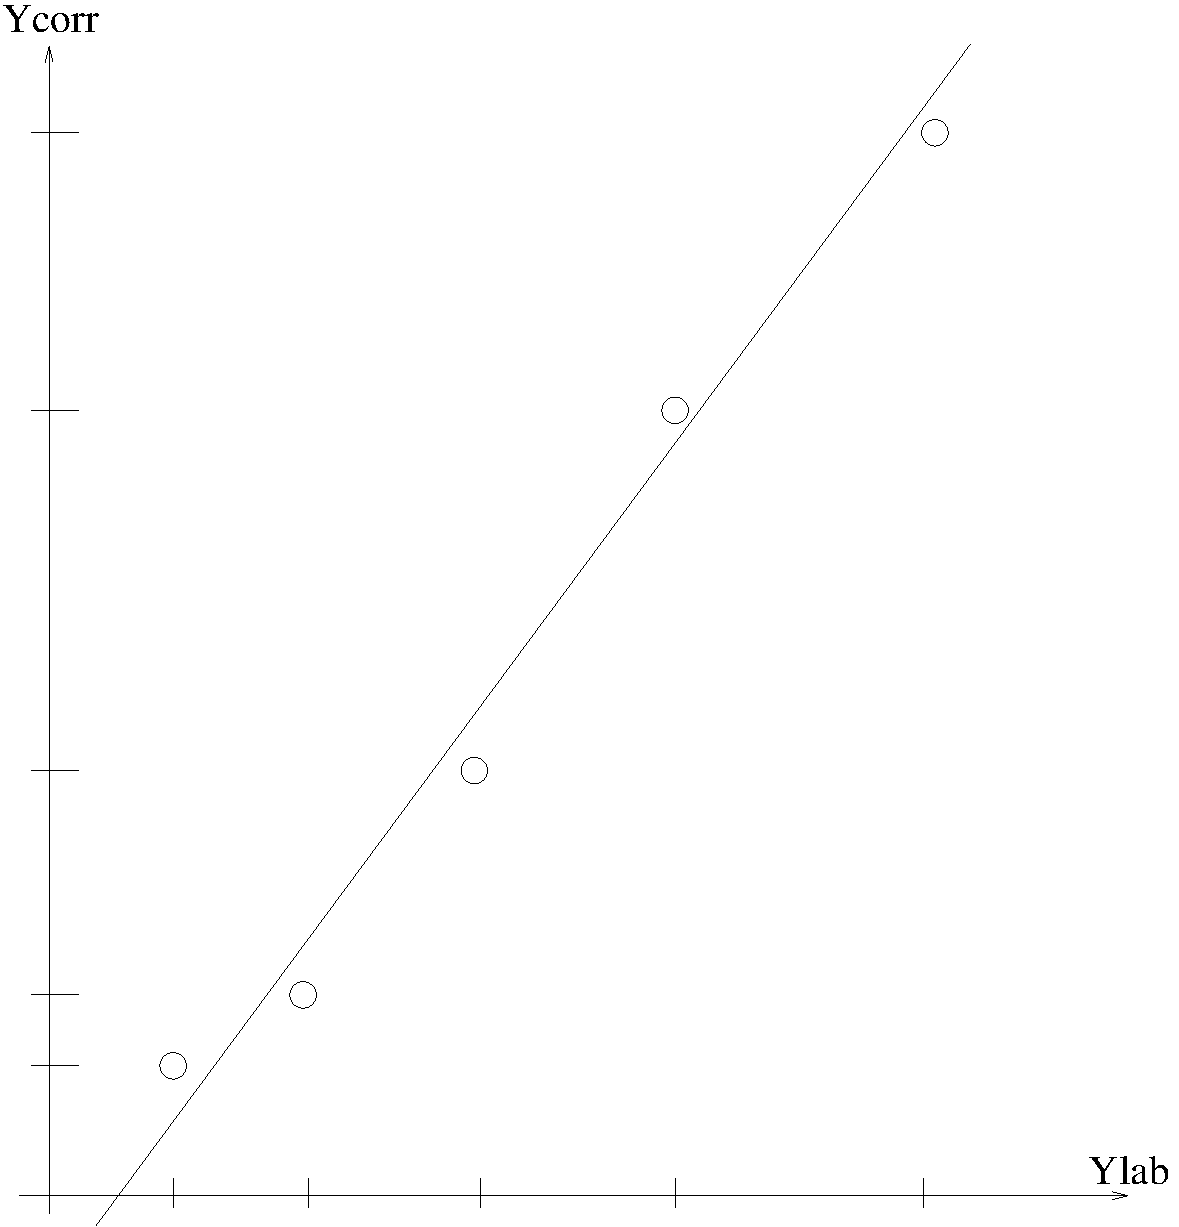
\includegraphics[scale=.25]{tuining}
   \begin{itemize}
    \item Recta por regresión sobre el error.
    \item Parámetros $c$ y $m$.
   \end{itemize}
  \end{column}
  \begin{column}{5cm}
   $Y_{ajusted} = c + m Y_{corr}$
   
    ~\

   Cómo decidir?
    \begin{itemize}
     \item $R^2$
     \item mse: suma de los errores al cuadrado.
     \item sigma ($\sigma$)
     \item $c$
     \item $m$
    \end{itemize}
  \end{column}
 \end{columns}
\end{frame}

\end{document}


